\documentclass[12pt]{article}

\usepackage[polish]{babel}
\usepackage{amsmath}
\usepackage{amsfonts}
\usepackage[skip=10pt plus1pt, indent=40pt]{parskip}

\usepackage{listings, listings-rust}
\usepackage{sourcecodepro}
\usepackage[T1]{fontenc}
\lstset{basicstyle=\ttfamily}

\usepackage{graphicx}

\graphicspath{ {assets/} }

\begin{document}
\begin{titlepage}
	\begin{center}
		\vspace*{1cm}
 
		{\huge \textbf{Równanie Transportu Ciepła}}
 
		\vspace{0.5cm}
		 Metoda Różnic Skończonych
			 
		\vspace{1.5cm}
 
		{\huge \textbf{Dominik Pilipczuk}}
 
		\vfill
			 
		Projekt obliczeniowy na przedmiot\\
		Równania Różniczkowe i Różnicowe
			 
		\vspace{0.8cm}
	
			 
		Akademia Górniczo Hutnicza w Krakowie\\
		21.01.2023
			 
	\end{center}
\end{titlepage}


\section{Wprowadzenie}
Celem projektu było rozwiązanie równania różniczkowego, podanego przez prowadzącego, metodą
 elementów skończonych. Zadanym problemem było równanie transportu ciepła w postaci:
\begin{equation}
	-k(x) \frac{d^2 u(x)}{dx^2} = 0
\end{equation}
gdzie:
\[
	k(x)=\begin{cases}
		1 & \text{dla $x \in [0,1]$}\\
		2 & \text{dla $x \in (1,2]$}
	  \end{cases}
\]
Samo równanie opisuje przepływ ciepła w układzie,
 uwzględniające różnice temperatury i właściwości cieplne materiałów. 
 Jest ono ważne w wielu dziedzinach, takich jak inżynieria cieplna czy fizyka.

\noindent Wraz z samym równaniem podane były warunki brzegowe:
\begin{equation}
	u(2)=0 
\end{equation}
oraz:
\begin{equation}
	\frac{du(0)}{dx} - u(0) = 20
\end{equation}
\noindent Łatwo zauważyć, że warunek (2) jest warunkiem Dirichleta dla $x = 2$, 
zaś warunek (3) jest warunkiem Cauchy'ego. Ponadto, dana jest dziedzina funkcji $u(x)$:
\[
	[0, 2] \ni x \to u(x) \in \mathbb{R}
\]




\newpage
\section{Obliczenia}
Przed wykorzystaniem narzędzi komputerowych do wyznaczenia funkcji $u$, 
 należy uprościć równanie (1), obliczając wzór na składniki $a$ i $L$:

\[
	-k \cdot u''(x) = 0	
\]
Dzielimy przez $-k(x) \ne 0$
\[
	u'' = 0	
\]
Wprowadzamy funkcję $v$, taką, że $v(2) = 0$, oraz całkujemy całe równanie:
\[
	\int_{0}^{2}u''\cdot v \,dx = 0
\]
Całkując przez części:
\[
	\left[ u' \cdot v  \right]_0^2 - \int_{0}^{2}u'\cdot v' \,dx = 0
\]
\[
	u'(2) \cdot v(2) - u'(0) \cdot v(0) - \int_{0}^{2}u'\cdot v' \,dx = 0
\]
Z (3) wyznaczamy wzór na $u'$, oraz odwracamy znaki:
\[
	\int_{0}^{2}u'\cdot v' \,dx + 20 \cdot v(0) - u(0) \cdot v(0) = 0
\]
\[
	\int_{0}^{2}u'\cdot v' \,dx - u(0) \cdot v(0) = -20 \cdot v(0)
\]
Wyznaczamy $a(u, v)$ oraz $L(v)$:
\begin{equation}
	a(u, v) = \int_{0}^{2}u'\cdot v' \,dx - u(0) \cdot v(0)
\end{equation}
\begin{equation}
	L(v) = -20 \cdot v(0)
\end{equation}

\newpage
\section{Implementacja}
Implementacji algorytmu MRS dokonałem w języku Rust, ponieważ zapewnia
on bezpieczeństwo, wydajność i elastyczność. 

\noindent Przy pisaniu programu wspomagałem się trzema bibliotekami
 odpowiedzialnymi za: wyliczanie całek, rozwiązanie układu macierzy oraz za
 stworzenie wykresu.

\noindent Całkowanie odbywa się za pomocą metody Gaussa-Legendre'a z czterema punktami kwadratury.

\noindent Całość kodu znajduje się w repozytorium na Githubie (podanym w komentarzu do zadania).

\subsection{Funkcje pomocnicze}
Zadeklarowałem parę pomocniczych funkcji, które po krótce opiszę.


\begin{lstlisting}[language=Rust, style=boxed]
fn get_a(u_d: impl Fn(f64) -> f64, 
	v_d: impl Fn(f64) -> f64,
	u: impl Fn(f64) -> f64, 
	v: impl Fn(f64) -> f64,
	a: f64, b: f64) -> f64 {
		
    let quad: GaussLegendre = 
		GaussLegendre::init(4);
		
    quad.integrate(a, b,
		|x| u_d(x)*v_d(x)) - u(0.)*v(0.)
}
\end{lstlisting}
\centerline{\textbf{get\_a} - zwraca $a(u,v)$}
\vskip 1cm

\begin{lstlisting}[language=Rust, style=boxed]
fn get_l(v: impl Fn(f64) -> f64) -> f64 {
	-20.0*v(0.0)
}
\end{lstlisting}
\centerline{\textbf{get\_l} - zwraca $L(v)$}

\begin{lstlisting}[language=Rust, style=boxed]
fn u_i(i_: usize) -> impl Fn(f64) -> f64{
	let n: f64 = N as f64;
	let i = i_ as f64;
	move |x| {
		if x > x_i(i - 1.) && x <= x_i(i) { 
			return n/2.0*x - i + 1.0
		}
		if x > x_i(i) && x < x_i(i+1.) { 
			return -n/2.0*x + i + 1.0
		};
		return 0.0;
	}
}
\end{lstlisting}
\centerline{\textbf{u\_i} - zwraca $u_i(x)$}
\vskip 1cm

\begin{lstlisting}[language=Rust, style=boxed]
fn ud_i(i_: usize) -> impl Fn(f64) -> f64 {
	let n = N as f64;
	let i = i_ as f64;
	move |x| {
		if x > x_i(i-1.) && x <= x_i(i) { 
			return n/2.0;
		}
		if x > x_i(i) && x < x_i(i+1.) { 
			return -n/2.0;
		};
		return 0.0;
	}
}
\end{lstlisting}
\centerline{\textbf{ud\_i} - zwraca $u'_i(x)$}
\vskip 1cm

\begin{lstlisting}[language=Rust, style=boxed]
fn x_i(i: f64) -> f64 {
	2.0*(i as f64)/(N as f64)
}
\end{lstlisting}
\centerline{\textbf{x\_i} - zwraca $x_i$}
\vskip 1cm

\noindent Ponadto, znajdują się funkcję tworzące wykres, w które szczegóły nie
 będę się zagłębiał.


\subsection{Funkcja główna}
\begin{lstlisting}[language=Rust, style=boxed, tabsize=2]
fn main() {
	// Macierz wypelniona zerami
	let mut a: Array2<f64> = 
		Array2::<f64>::zeros((N+1, N+1)); 

	let n = N as f64;
	// Wypelniamy macierz zgodnie z 
	// przykladem na zajeciach
	for i in 0..N {
		for j in 0..=N {
			let s: f64;
			let e: f64;
			let diff = i.abs_diff(j); 
			if diff > 1 { continue; }
			if diff == 1 {
				s = 2. * f64::max(0.,
					f64::min(i as f64, j as f64) / n);

				e = 2. * f64::min(1.,
					f64::max(i as f64, j as f64) / n);
			} else {
				s = 2. * f64::max(0., (i as f64 - 1.) / n);
				e = 2. * f64::min(1., (i as f64 + 1.) / n);
            }


			a[[i, j]] = get_a(ud_i(j), ud_i(i),
				u_i(j), u_i(i), s, e);
		}
	}

	a[[N, N]] = 1.;

	// Macierz B
	let mut b: Array1<f64> =
		Array1::<f64>::zeros(N+1);

	for i in 0..N {
		b[i] = get_l(u_i(i));
	}
	b[N] = 0.;

	// Rozwiazujemy uklad macierzy
	let res = a.solve_into(b).unwrap();
    
	// tworzymy punkty
	let x: Vec<f64> = (0..=2000)
	.map(|x| x as f64*0.001).
	collect::<Vec<f64>>();

	let mut y = vec![0f64; x.len()];

	for i in 0..x.len() {
		for j in 0..res.len() {
			let e = u_i(j);
			y[i] = y[i] + res[j] * e(x[i])
		}
	}

	// rysujemy wykres
	plot(x, y);
}	
\end{lstlisting}

\noindent Funckja $main()$ działa analogicznie do przykładów podanych na zajęciach.
Tworzy i wypełnia macierz $A$ i $B$ po czym rozwiązuje układ równań $A\cdot X = B$
i ukazuje wyniki na wykresie.

\newpage

\section{Wyniki}
Po uruchomienu programu w konsoli powinny wyświetlić się przybliżone wartości macierzy (zaokrąglone do pierwszego miejsca po przecinku), oraz okno z wyznaczonym wykresem.

\noindent Warto zaznaczyć, że zaokrąglenia mają jedynie na celu ułatwić czytanie, zatem nie 
mają wpływu na przeprowadzane obliczenia.


\vskip 1cm
\begin{center}
	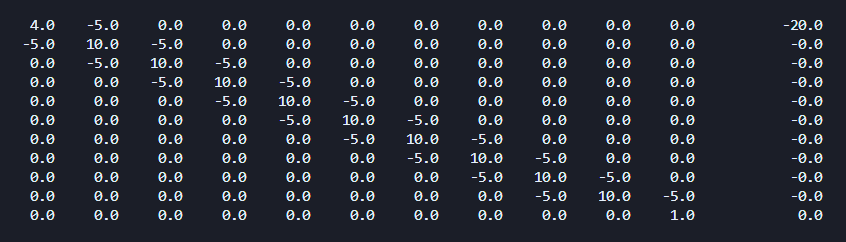
\includegraphics[width=\textwidth]{matrix_ab.png}

	\textbf{Rysunek 1.} Układ równań.
\end{center}

\vskip 1cm
\begin{center}
	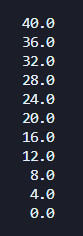
\includegraphics[]{matrix_c.png}

	\textbf{Rysunek 2.} Rozwiązanie układu równań (1).
\end{center}

\vskip 1cm
\begin{center}
	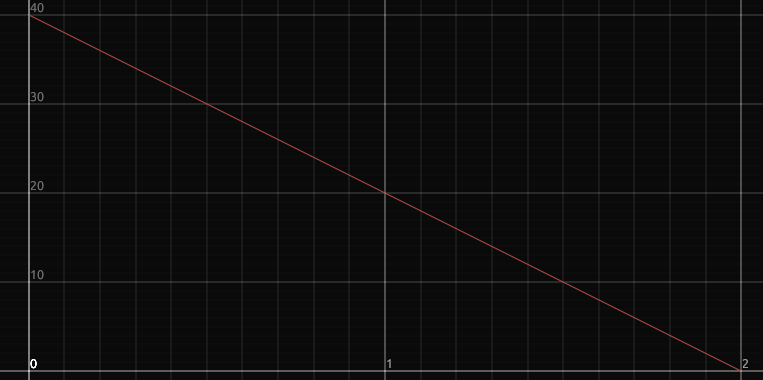
\includegraphics[width=\textwidth]{chart.png}

	\textbf{Rysunek 3.} Wykres wyliczonej funkcji.
\end{center}

\newpage
\section{Wnioski}
Po przeanalizowaniu wykresu funkcji $u(x)$ możemy wyznaczyć jej wzór:
\begin{equation}
	u(x) = -20x + 40
\end{equation}

\subsection{Dowód}
Dla pewności, możemy podstawić wyznaczoną funkcję pod otrzymane równości i udowodnić jej poprawność.

\noindent Ze wzoru (1) wiemy, że funkcja $u$ jest ciągła (bądź nie zależy w ogóle od $x$), 
ponieważ jej druga pochodna $u''(x)$ jest równa zeru.

\noindent Ponadto, funkcja $u(x)=-20x+40$ spełnia warunek Dirichleta (2) i warunek Cauchy'ego (3).

\end{document}